O desenvolvimento do projeto incluiu diversas tecnologias, sendo as principais a linguagem de Programação \emph{R} e o middleware
para computação voluntária \emph{Boinc}. Dentre os conceitos estudados, 

\subsection{BOINC}

%Fonte wikipedia

O BOINC, cujo nome é uma sigla para \textit{Berkeley Open Infrastructure for Network Computing}, é um middleware 
para computação em grade e voluntária e foi criado na Universidade de Berkeley, Califórnia, Estados Unidos.

Inicialmente, o projeto consistia em gerenciar o projeto \textit{SETI@HOME} que possuía dois objetivos:

\begin{itemize}
	\item Provar a viabilidade e a praticidade do conceito ``computação em grade distribuída'';
	\item Fazer um trabalho científico útil fazendo uma análise observacional para detectar vida inteligente fora da Terra.
\end{itemize}

O primeiro objetivo foi concluído com sucesso e o resultado é o \textit{BOINC}. O segundo falhou: nenhuma evidência de 
vida inteligente fora da Terra foi encontrada. 

\subsubsection{Funcionamento do BOINC}

Cada unidade de processamento no Boinc é chamada de \emph{workunit} e é constítuida de arquivos executáveis e 
arquivos de entrada. Depois de processado, os arquivos de saída gerados são enviados para o servidor que
normalmente armazena estes arquivos em um banco de dados ou em um arquivo.

Para gerar um workunit são necessários dois arquivos XML, um deles detalhando a entrada e o 
outro detalhando a saída. Para facilitar a escrita do programa, precisamos escrever para cada arquivo um nome lógico 
que ao enviar e receber o cliente renomeia o arquivo. Por exemplo, temos um programa que lê um arquivo chamado 
\verb#input# e escreve no arquivo \verb#output#, para podermos ter muitos arquivos de entrada com nomes diferentes, quando
criamos uma \emph{workunit}, o servidor coloca um nome único e semelhante ao da workunit nos arquivos de entrada e saída que serão renomeados
pelo cliente para o nome lógico.

O processamento é realizado pelo cliente: o arquivo binário é executado e enquanto ele é executado há um checkpoint
que permite em caso de interrupções retomar o processamento de um determinado ponto. Finalizado o processamento, 
na próxima atualização o cliente avisará ao servidor que o processamento foi finalizado. Um diagrama do funcionamento pode
ser visto na figura \ref{funcionamento-boinc}. 


\begin{figure}[!h]
  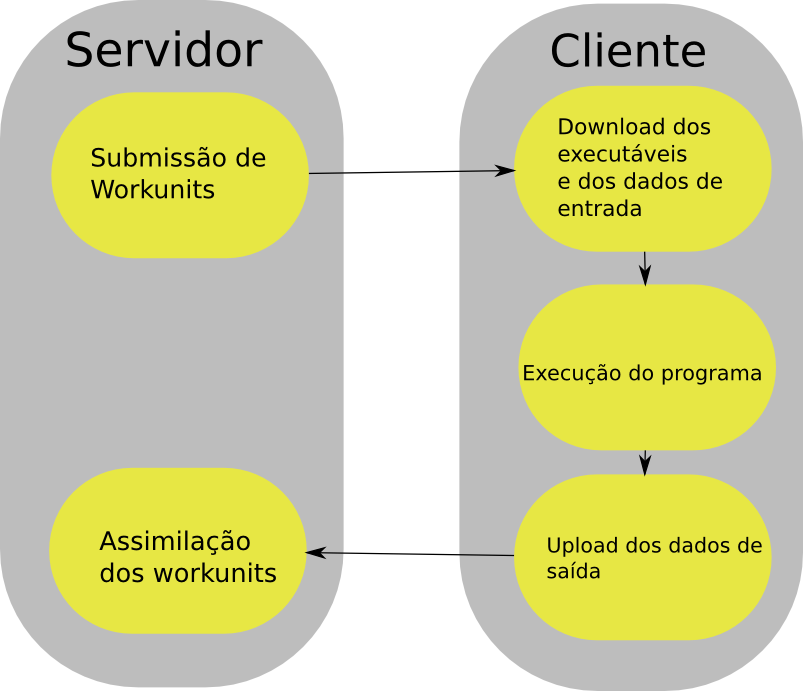
\includegraphics[scale=0.5]{boinc-schema.png}
  \caption{Funcionamento do Boinc}
  \label{funcionamento-boinc}
\end{figure}


\subsubsection{Wrapper}

%Fonte: página do Wrapper no site do BOINC

O \emph{Wrapper} é um programa escrito utilizando a \emph{api} do \emph{BOINC}, cujo objetivo é executar aplicações legadas, 
i.e. aplicações que não utilizam a API do \emph{BOINC}, utilizando o \textit{BOINC}. Há uma versão do Wrapper distribuída junto com o 
\textit{BOINC} que utiliza um arquivo XML, mas existe uma outra opção descrita no artigo %Artigo do Húngaro
que utiliza um shell para a execução dos aplicativos.

O arquivo XML de execução tem a seguinte estrutura:

\begin{verbatim}
<job_desc>
    <task>
        <application>foobar</application>
        [ <stdin_filename>stdin_file</stdin_filename> ]
        [ <stdout_filename>stdout_file</stdout_filename> ]
        [ <stderr_filename>stderr_file</stderr_filename> ]
        [ <command_line>--foo bar</command_line> ]
    </task>
    [ ... ]
</job_desc>
\end{verbatim}

Neste XML, o único campo obrigatório é o \emph{application}, que é a aplicação
que será executada e pode ser distribuída junto com a aplicação ou já existir no 
computador que o cliente estará instalado (para este segundo caso é necessário
informar o caminho inteiro do executável). É possível ter mais de uma tag
task, e o wrapper as executará sequencialmente. É de responsabilidade
do \textit{Wrapper} 

\subsection{R}

%Fonte wikipedia

A linguagem de programação estatística $R$ é uma implementação da linguagem $S$ e foi criada por John Ihaka e Robert
Gentleman na Universidade de Auckland, da Nova Zelândia. Hoje, a linguagem $R$ é uma linguagem considerada padrão
entre estatísticos no desenvolvimento de softwares estatísticos e na análise de dados. Há também um ambiente 
onde podemos utilizar a linguagem em um interpretador e gerar gráficos de alta qualidade. 

Por padrão, as distribuições estatísticas mais populares podem ser utilizadas e é muito mais simples que em 
linguagens como C, Java a manipulação de matrizes e tabelas de dados.Outro ponto importante na linguagem $R$ 
é a extensibilidade: é muito simples instalar bibliotecas. Hoje em dia, há
cerca de $2000$ bibliotecas no repositório principal (chamado de \emph{CRAN}, 
sigla de \textit{Comprehensible R Archive Network}) com as mais diversas funções 
(desde bibliotecas de gráficos específicos até métodos estatísticos mais complexos). 
Outro repositório bastante utilizado é o Bioconductor, que provê rotinas bastante utilizadas para o processamento
de dados da área de bioinformática.




